\chapter{Margin Maximization}
\label{chap-margin}

\section{Machine learning as optimization}
The perceptron algorithm was originally written down directly via
cleverness and intuition, and later analyzed theoretically. Another
approach to designing machine learning algorithms is to frame them as
optimization problems, and then use standard optimization algorithms
and implementations to actually find the hypothesis.

We begin by writing down an \emph{objective function} $J(\Theta)$,
where $\Theta$ stands for {\em all} the parameters in our model.
Note that we will sometimes write $J(\theta, \theta_0)$
because when studying linear classifiers, we have used these two
names for parts of our whole collection of parameters, so $\Theta =
(\theta, \theta_0)$.
We also often write $J(\Theta; \data)$ to make clear the dependence on
the data $\data$.  The objective
function describes how we feel about
possible hypotheses $\Theta$: we will generally look for values for
parameters $\Theta$ that minimize the objective function:
\note{You can think about $\Theta^*$ here as ``the theta that
  minimizes $J$''.} 
\[ \Theta^* = \argmin{\Theta} J(\Theta)\;\;. \]

A very common form for an ML objective is
\[
  J(\Theta) = \left(\frac{1}{n} \sum_{i=1}^n
    \underbrace{L(h(\ex{x}{i}; \Theta), 
  \ex{y}{i})}_\text{loss}\right) + \underbrace{\lambda}
  _\text{constant} \underbrace{R(\Theta)}_\text{regularizer}.
\]
The \emph{loss} tells us how unhappy we are about the prediction
$h(\ex{x}{i}; \Theta)$ that
$\Theta$ makes for $(\ex{x}{i}, \ex{y}{i})$. A common example
is the 0-1 loss, introduced in Chapter~\ref{chap-intro}:
\[ L_{01}(h(x; \Theta), y) =
  \begin{cases}
    0 & \text{ if } y = h(x; \Theta)\\
    1 & \text{ otherwise}
  \end{cases}
\]
which gives a value of 0 for a correct prediction, and a 1 for an
incorrect prediction.  In the case of linear separators, this becomes:
\[ L_{01}(h(x;\theta, \theta_0), y) =
  \begin{cases}
    0 & \text{ if } y(\theta^Tx + \theta_0) > 0 \\
    1 & \text{ otherwise}
  \end{cases}
\]

\section{Regularization}

If all we cared about was finding a hypothesis with small loss on the
training data, we would have no need for regularization, and could
simply omit the second term in the objective.  But remember that our
objective is to {\em perform well on input values that we haven't
  trained on!}  It may seem that this is an impossible task, but
humans and machine-learning methods do this successfully all the
time.  What allows {\em generalization} to new input values is a
belief that there is an underlying regularity that governs both the
training and testing data.  We have already discussed one way to
describe an assumption about such a regularity, which is by choosing a
limited class of possible hypotheses.  Another way to do this is to
provide smoother guidance, saying that, within a hypothesis class, we
prefer some hypotheses to others.  The regularizer articulates this
preference and the constant $\lambda$ says how much we are willing to
trade off loss on the training data versus preference over hypotheses.

This trade-off is illustrated in the figure below.  Hypothesis $h_1$
has 0 training loss, but is very complicated.  Hypothesis $h_2$
mis-classifies two points, but is very simple.  In absence of other
beliefs about the solution, it is often better to prefer that the
solution be ``simpler,'' and so we might prefer $h_2$ over $h_1$,
expecting it to perform better on future examples drawn from this same
distribution.  \note{To establish some vocabulary, we might say that
  $h_1$ is {\em overfit} to the training data.}  Another nice way of
thinking about regularization is that we would like to prevent our
hypothesis from being too dependent on the particular training data
that we were given: we would like for it to be the case that if the
training data were changed slightly, the hypothesis would not change
by much.

\begin{center}
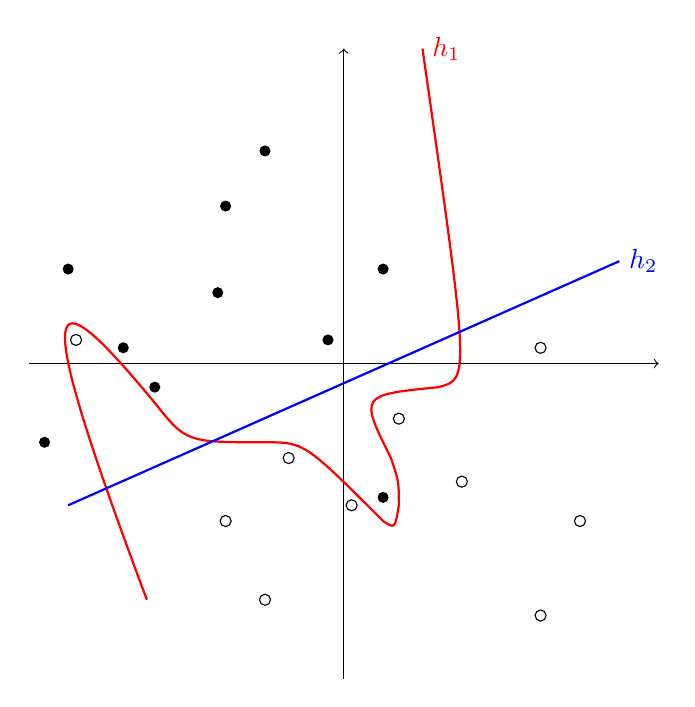
\begin{tikzpicture}
  \draw [->] (-4,0) -- (4,0);
  \draw [->] (0,-4) -- (0,4);
  \draw[red,thick] (-2.5,-3) .. controls (-4,1) and (-3.8,1.2) .. (-2.4,-.5)
    .. controls (-2,-1) .. (-1,-1) .. controls (-.5,-1) ..  (.5,-2)
    .. controls (.65, -2.1) .. (.7,-1.8) .. controls (.7,-1.5)
    ..  (.6,-1.2) .. controls (.2,-.4) .. (1.2, -.3)
    .. controls (1.6,-.2) .. (1,4);

  \foreach \Point in {(-3.4, .3), (2.5, .2), (-1.5,-2), (-1,-3),(.7,-.7),
    (3, -2), (2.5, -3.2), (-.7,-1.2), (0.1,-1.8), (1.5, -1.5)}{
    \draw \Point circle[radius=2pt];
  }
  \foreach \Point in {(.5,-1.7),(-.2,.3),(-2.8,.2),(-2.4,-.3),(-1,2.7),
    (-1.5, 2), (-1.6, .9), (-3.8,-1), (-3.5,1.2),(.5, 1.2)}{
  \fill \Point circle[radius=2pt];
  }
  \draw[blue, thick] (-3.5,-1.8) -- (3.5,1.3);
  \node[right,blue] at (3.5,1.3) {$h_2$};
  \node[below,right,red] at (1,4) {$h_1$};

\end{tikzpicture}
\end{center}

A common strategy for specifying a \emph{regularizer} is to use the form
\[ R(\Theta) = \norm{\Theta - \Theta_{\it prior}}^2 \]
when we have some idea in advance that $\theta$ ought to be near some
value $\Theta_{\it prior}$.  
\note{Learn about Bayesian methods in machine learning to see the
  theory behind this and cool results!}
In the absence of such knowledge a default is
to {\em regularize toward zero}:
\[ R(\Theta) = \norm{\Theta}^2\;\;. \]

\section{Maximizing the margin}
One criterion to use for judging separators that classify all
examples correctly (that is, that have a 0-1 loss value of 0) is to
prefer ones that have a {\em large margin}.
Recall that the margin of a labeled point $(x,y)$
with respect to the hyperplane $\theta, \theta_0$ is
\[ \gamma(x,y,\theta,\theta_0) = \frac{y\left(\theta^Tx+\theta_0\right)}
{\norm{\theta}} \;\;.\]
The margin is positive if a point is classified correctly, and the
absolute value of the margin is the perpendicular distance of $x$ to the
hyperplane. The margin of a dataset $\data$ with respect to
$\theta,\theta_0$ is
\[ 
  \min_{(\ex{x}{i},\ex{y}{i})\in \data}
  \gamma(\ex{x}{i},\ex{y}{i},\theta,\theta_0)\;\;.
\]
The figure below illustrates the margin of two linear separators, each
with 0 loss, with respect to the same data set.  The separator, $h_1$,
with the larger margin $\gamma_1$ feels intuitively like it will have
better generalization performance.  Separator $h_2$ has a very small
margin and would make errors if the data were perturbed by a small
amount.  \note{There is a lot of interesting theoretical work
  justifying a preference for separators with large margin.  There is
  an important class of algorithms called {\it support vector
    machines} that focus on finding large-margin separators with some
  other interesting properties.  Before the current boom in neural
  networks, they were the ``go-to'' algorithms for classification.  We
  don't have time to study them in more detail in this class, but we
  recommend that you read about them some time.}

\begin{center}
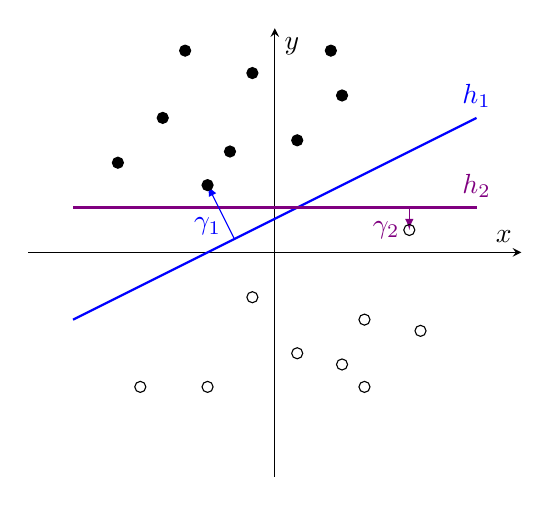
\begin{tikzpicture}
\begin{axis}[
    axis lines=middle, axis equal image,
    xmin=-11, xmax=11,
    ymin=-10, ymax=10,
    xtick=\empty, ytick=\empty,
    xlabel={$x$}, ylabel={$y$}
]
\addplot [only marks] table {
-3  3
1   5
-5  6
-1  8
3   7
-2  4.5
-7  4
-4  9
2.5 9
};
\addplot [only marks, mark=o] table {
-1  -2
-3  -6
4   -3
1   -4.5
3   -5
6   1
4   -6
6.5 -3.5
-6  -6
};
\addplot [domain=-9:9, samples=2, thick, blue] {.5*x+1.5} node[above] {$h_1$};
\addplot [domain=-9:9, samples=2, thick, violet] {2} node[above] {$h_2$};
\draw [latex-,blue] (axis cs: -3, 3) node [blue,yshift=-1.5em] {$\gamma_1$}
  -- (axis cs: -1.8, .6);
\draw [latex-,violet] (axis cs: 6, 1) node [violet,left] {$\gamma_2$}
  -- (axis cs: 6, 2);
\end{axis}
\end{tikzpicture}
\end{center}

If our data is linearly separable, we can frame the problem of finding
the maximum-margin separator as
\[
  \theta^*, \theta_0^* = \argmax{\theta,\theta_0} \min_i \gamma(\ex{x}{i},
  \ex{y}{i},\theta,\theta_0)\;\;,
\]
which we can find by minimizing the objective
\[
  J(\theta,\theta_0) = -\min_i \gamma(\ex{x}{i},\ex{y}{i},\theta,
  \theta_0)\;\;.
\]
However, this form of the objective can be tricky to optimize because
it is only sensitive to a single data point at a time, and so gradient
methods won't work very well.\note{This remark won't make sense to you
  until you understand more about gradient methods---so come back to
  think about it after you read the next chapter.}

We will develop another formulation.  Let's start by assuming
that we can guess what a good target value would be for the margin,
and call it $\gamma_{\it ref} > 0$. We can then set up a problem in
which we try to find a separator with margin $\gamma_{\it ref}$.
Ultimately, our goal will be to find a value for $\gamma_{\it ref}$
and a separator such that:
\begin{itemize}
  \item all points have margin $> \gamma_{\it ref}$ and
  \item the target margin $\gamma_{\it ref}$ is big.
\end{itemize}

\noindent To make this more precise, we start by defining a new loss function
\note{Confusion alert:  we have told you that loss functions are a
  function of two arguments, a guessed value and an actual value, but
  this ``loss function'' has a single argument, which is a margin.  A
  margin already combines the guess
  $\theta^Tx+\theta_0 / \norm{\theta}$ with the actual value
  $y$.  This is a standard way of framing the problem in the ML world,
  so we will stick with it.}
called the {\em hinge loss}:
\[
  L_h (\gamma / \gamma_{\it ref}) =
    \begin{cases}
      1 - \gamma / \gamma_{\it ref} & \text{ if } \gamma < \gamma_{\it ref} \\
      0 & \text{ otherwise}
    \end{cases}\;\;.
\]
The figure below and to the left plots the hinge loss as a function of
the margin, $\gamma$, of a point.  It is zero if the margin is greater
than $\gamma_{\it ref}$ and increases linearly as the margin decreases
(because we {\em really} want the margin to be bigger than
$\gamma_{\it ref}$!).
\begin{center}
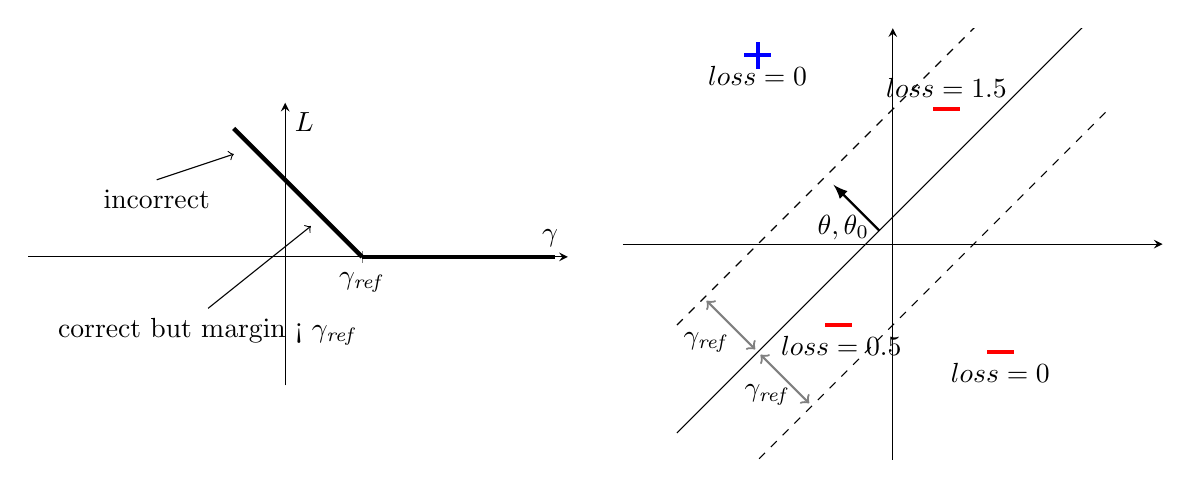
\begin{tikzpicture}
\begin{axis}[
    name=left,
    axis lines=middle, axis equal image,
    xmin=-10, xmax=11,
    ymin=-5, ymax=6,
    xtick={3}, ytick=\empty,
    xticklabels={$\gamma_{\it ref}$},
    xlabel={$\gamma$}, ylabel={$L$},
]
\addplot [domain=-2:3, samples=2, ultra thick] {3-x}; 
\addplot [domain=3:10.5, samples=2, ultra thick] {0};
\draw [->] (axis cs: -5, 3) node [black,below] {incorrect}
  -- (axis cs: -2, 4);
\draw [->] (axis cs: -3, -2) node [black,below] {correct but
  margin < $\gamma_{\it ref}$}
  -- (axis cs: 1, 1.2);

\end{axis}
\begin{axis}[
    axis lines=middle, axis equal image,
    xmin=-10, xmax=10,
    ymin=-8, ymax=8,
    xtick=\empty, ytick=\empty,
    at = (left.east), anchor = west, xshift = .7cm
]
\addplot [domain=-8:8, samples=2] {x+1}; 
\addplot [domain=-8:8, samples=2,dashed] {x+5};
\addplot [domain=-8:8, samples=2,dashed] {x-3};
\draw [thick,-latex] (axis cs: -0.5, 0.5) node [black,left,yshift=.1em]
  {$\theta,\theta_0$} -- (axis cs: -2.2, 2.2) ;
  
  \draw[ultra thick, blue] +(axis cs: -5-.5,7) -- +(axis cs: -5+.5,7)
    node [black,below,xshift=-.5em] {$loss=0$};
  \draw[ultra thick, blue] +(axis cs: -5,7-.5) -- +(axis cs: -5,7+.5);

  \draw[ultra thick, red] +(axis cs: 2-.5,5) -- +(axis cs: 2+.5,5)
    node [black,above,xshift=-.5em] {$loss=1.5$};
  \draw[ultra thick, red] +(axis cs: -2-.5,-3) -- +(axis cs: -2+.5,-3)
    node [black,below,xshift=-.4em] {$loss=0.5$};
  \draw[ultra thick, red] +(axis cs: 4-.5,-4) -- +(axis cs: 4+.5,-4)
    node [black,below,xshift=-.5em] {$loss=0$};

  \draw[<->, gray, thick] (axis cs: -5.1,-3.9) -- (axis cs: -6.9, -2.1)
    node [black,yshift=-1.5em] {$\gamma_{\it ref}$};
  \draw[<->, gray, thick] (axis cs: -4.9,-4.1) -- (axis cs: -3.1, -5.9)
    node [black,yshift=.3em,xshift=-1.5em] {$\gamma_{\it ref}$};
\end{axis}
\end{tikzpicture}
\end{center}

\question{Plot 0-1 loss on the axes of the figure on the left.}

In the figure on the right, we illustrate a hyperplane $\theta, \theta_0$.
Parallel to that hyperplane, but offset in either direction by
$\gamma_{\it ref}$ are two more hyperplanes (dotted lines in the
figure) representing the margins.  Any correctly classified point
outside the margin has loss 0.  Any correctly classified point inside
the margin has loss in $(0, 1)$.  Any incorrectly classified point has
loss $\geq 1$.  
\question{Be sure you can compute the loss values shown on this
  figure.  Also, try to visualize a plot in 3 dimensions that shows
  the loss function for positive points and the loss function for
  negative points going in the $Z$ dimension (up out of the page) on
  top of this plot.}

Now, let's formulate an objective function, in terms of the parameters
$\Theta = (\theta, \theta_0, \gamma_{\it ref})$.  
We will express our desire for a large margin by employing a regularization 
term in the objective function, namely
$R(\theta,\theta_0, \gamma_{\it ref}) = 1/\gamma_{\it 
    ref}^2$. \note{If you are thinking to yourself that we could
  express the desire for large margin by setting $R = -\gamma_{\it ref}$ or $R =
  1/\gamma_{\it ref}$ or any of a variety of other things, you would be right.
  We'll insist on this choice for now, because it will turn out to
  have useful consequences later, but you have no way of seeing that
  at this point.}
Then, we have 
\[
  J(\theta,\theta_0,\gamma_{\it ref}) = \frac{1}{n}\sum_{i=1}^n
  L_h\left(\frac{\gamma(\ex{x}{i},\ex{y}{i},\theta,\theta_0)}{\gamma_{\it ref}}
  \right) + \lambda\left(\frac{1}{\gamma_{\it ref}^2}\right)\;\;.
\]
We see that the two terms in the objective function have opposing
effects, favoring small and large $\gamma_{\it ref}$, respectively,
with $\lambda$ \note{Because it's not a parameter of the hypothesis,
  but rather a parameter of the method we are using to choose the
  hypothesis, we call $\lambda$ a {\em hyperparameter.}}  governing
the trade-off.  
\question{ You should, by now, be asking yourself
  ``How do we pick $\lambda$?''  You can think of the different
  objective functions that result from different choices of
  hyperparameter $\lambda$ as different {\em learning algorithms}.
  What do you know about choosing among algorithms?  How would you use
  that to pick $\lambda$?
}

Now, in order to slightly simplify our problem and to connect up with
more standard existing methods, we are going to make a somewhat
unintuitive step.  \note{This is kind of tricky.  Stew about it until
  it  makes sense to you.}
We actually have one more parameter in our set of parameters
$(\theta, \theta_0, \gamma_{\it ref})$ than is really necessary for
describing our hypothesis and objective, so we are going to rewrite it.

Remember that any linear scaling of $\theta,\theta_0$
represents the same separator.  So, without losing any ability to
represent separators or describe their margins, 
we can scale $\theta, \theta_0$ so that 
\[ \norm{\theta} = \frac{1}{\gamma_{\it ref}}\;\;. \]
\note{It's like we're secretly encoding our target margin as the
  inverse of the norm
  of $\theta$.}
Note that, because our target margin scales inversely with
$\norm{\theta}$, wanting the margin to be large is the same as wanting
$\norm{\theta}$ to be small.

With this trick, we don't need $\gamma_{\it ref}$ as a parameter any
more, and we get the following objective, which is the objective
  for support vector machines, and we'll often refer to as the 
SVM objective:
\[ J(\theta,\theta_0) = \left(\frac{1}{n}\sum_{i=1}^n L_h\left(\ex{y}{i}
(\theta^Tx+\theta_0)\right)\right) + \lambda\norm{\theta}^2 \;\;.\]
For any linearly separable data set, here are some observations:
\begin{enumerate}
  \item If $\lambda = 0$, $\theta, \theta_0$ can always
    be chosen so that the objective function evaluates to 0.
  \item If $\lambda > 0$ but is very small, we will pick $\theta$
    with smallest $\norm{\theta}$ while still maintaining separation
    of the data.
  \item If $\lambda$ is large, we tolerate errors in favor of having a
    ``simpler'' (smaller norm) separator.
\end{enumerate}
\question{Be sure you can make a detailed explanation of each of these
  points.   In point 1 above, would we need to increase or decrease the
  magnitude of $\theta$ to make the objective go to zero?  How does
  point 3 relate to the idea of regularizing toward zero?}

At the optimum, for separable data with very small $\lambda$:
\begin{itemize}
  \item $\ex{y}{i}\left(\theta^T\ex{x}{i} + \theta_0\right) \geq 1$ for
  all $i$, so as to keep the hinge loss to 0 for all points.
  \item $\ex{y}{i}\left(\theta^T\ex{x}{i} + \theta_0\right) = 1$ for
  at least one $i$, because the regularizer will drive $\norm{\theta}$ to be
  as small as possible with the loss still remaining at 0. 
\end{itemize}
To understand this, we note that
points for which $\ex{y}{i}\left(\theta^T\ex{x}{i} + \theta_0\right) = 1$
have margin exactly equal to $\gamma_\text{ref}$ (otherwise we could decrease
  $\norm{\theta}$ to obtain a larger margin). For these points that lie
  along the margin, we use the signed distance from $\theta,\theta_0$ to the point to
  compute the margin of this separator with respect to the data set:
  \[ \frac{\ex{y}{i}\left(\theta^T\ex{x}{i}+\theta_0\right)}
    {\norm{\theta}} = \text{margin}\;\;,\]
and so 
 \[\text{margin} =\frac{1}{\norm{\theta}} \;\;.\]

\note{Note that this last assertion (that the margin is the inverse of
  the norm of $\theta$) is only true under the assumptions listed at
  the top of this paragraph:  when the data is separable, when
  $\lambda$ is very small, and when $\theta$ is the optimum of the SVM
  objective.}  
\question{Be sure you can derive this last step and understand the
  conditions under which it holds!}


%%% Local Variables:
%%% mode: latex
%%% TeX-master: "top"
%%% End:
